\documentclass[tikz,border=4pt]{standalone}
\usepackage[T1]{fontenc}
\usepackage{lmodern}
\usepackage{amsmath}
\usepackage{amssymb}
\usetikzlibrary{arrows.meta,positioning,calc,shapes.geometric,fit,backgrounds}

\begin{document}
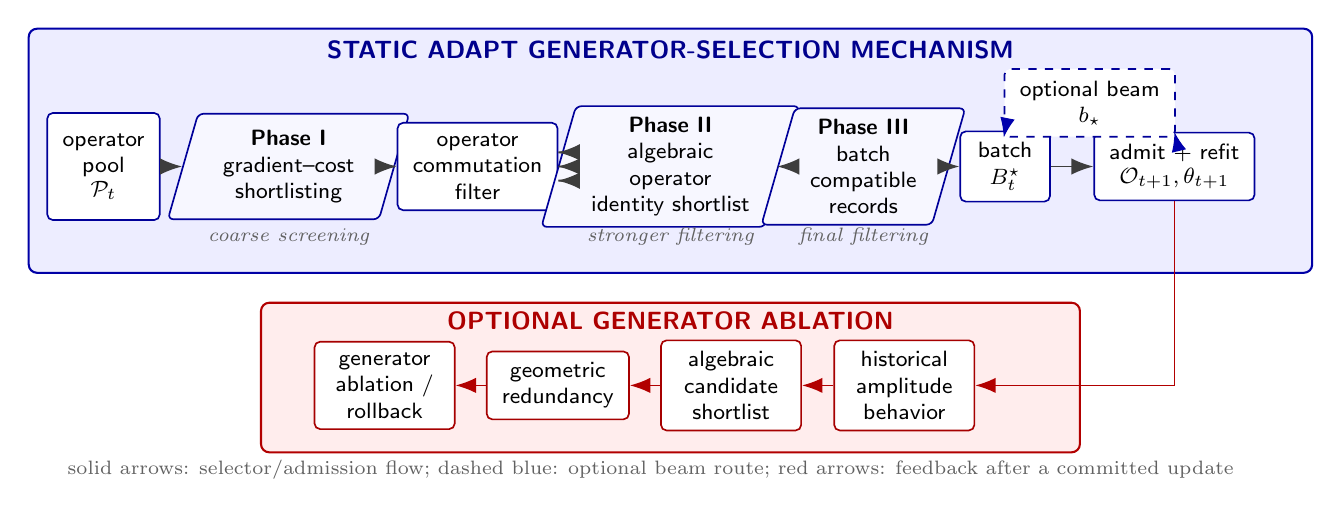
\begin{tikzpicture}[
  font=\sffamily\footnotesize,
  box/.style={
    draw=blue!60!black,
    line width=0.60pt,
    rounded corners=2.0pt,
    fill=white,
    align=center,
    minimum height=0.86cm,
    inner xsep=5.5pt,
    inner ysep=4.0pt
  },
  redbox/.style={
    box,
    draw=red!65!black,
    fill=white
  },
  phase/.style={
    box,
    trapezium,
    trapezium left angle=74,
    trapezium right angle=106,
    fill=blue!3
  },
  arrow/.style={-{Latex[length=2.8mm]}, line width=0.68pt, draw=black!76},
  feedback/.style={-{Latex[length=2.6mm]}, line width=0.62pt, draw=red!70!black},
  opt/.style={-{Latex[length=2.5mm]}, dashed, line width=0.62pt, draw=blue!68!black},
  title/.style={font=\sffamily\bfseries\small, align=center},
  note/.style={font=\scriptsize, text=black!62, align=center}
]

\node[draw=blue!65!black, rounded corners=3pt, line width=0.75pt,
      fill=blue!7, minimum width=16.30cm, minimum height=3.10cm] (bluepanel) at (7.20,0.42) {};
\node[draw=red!70!black, rounded corners=3pt, line width=0.75pt,
      fill=red!7, minimum width=10.40cm, minimum height=1.90cm] (redpanel) at (7.20,-2.46) {};

\node[title, text=blue!55!black] at (bluepanel.north) [yshift=-0.28cm]
  {STATIC ADAPT GENERATOR-SELECTION MECHANISM};
\node[title, text=red!68!black] at (redpanel.north) [yshift=-0.24cm]
  {OPTIONAL GENERATOR ABLATION};

\node[box, minimum width=1.36cm, minimum height=1.36cm] (pool) at (0,0.22)
  {operator\\pool\\[-1pt]$\mathcal P_t$};
\node[phase, minimum width=2.62cm, minimum height=1.34cm] (p1) at (2.35,0.22)
  {\textbf{Phase I}\\gradient--cost\\shortlisting};
\node[box, minimum width=1.56cm] (comm) at (4.75,0.22)
  {operator\\commutation\\filter};
\node[phase, minimum width=2.34cm, minimum height=1.18cm] (p2) at (7.20,0.22)
  {\textbf{Phase II}\\algebraic\\operator\\identity shortlist};
\node[phase, minimum width=2.06cm, minimum height=1.04cm] (p3) at (9.65,0.22)
  {\textbf{Phase III}\\batch\\compatible\\records};
\node[box, minimum width=1.14cm] (batch) at (11.45,0.22)
  {batch\\$B_t^\star$};
\node[box, minimum width=1.72cm] (admit) at (13.60,0.22)
  {admit + refit\\[-1pt]$\mathcal O_{t+1},\theta_{t+1}$};
\coordinate (beamcenter) at ($(batch.north)!0.5!(admit.north)$);
\node[box, dashed, minimum width=1.58cm] (beam) at ($(beamcenter)+(0,0.36)$)
  {optional beam\\$b_\star$};

\node[redbox, minimum width=1.78cm] (ablate) at (3.57,-2.56)
  {generator\\ablation /\\rollback};
\node[redbox, minimum width=1.78cm] (geom) at (5.77,-2.56)
  {geometric\\redundancy};
\node[redbox, minimum width=1.78cm] (alg) at (7.97,-2.56)
  {algebraic\\candidate\\shortlist};
\node[redbox, minimum width=1.78cm] (hist) at (10.17,-2.56)
  {historical\\amplitude\\behavior};

\draw[arrow] (pool) -- (p1);
\draw[arrow] (p1) -- (comm);
\draw[arrow] ($(comm.east)+(0,0.18)$) -- ($(p2.west)+(0,0.18)$);
\draw[arrow] (comm.east) -- (p2.west);
\draw[arrow] ($(comm.east)+(0,-0.18)$) -- ($(p2.west)+(0,-0.18)$);
\draw[arrow] (p2) -- (p3);
\draw[arrow] (p3) -- (batch);
\draw[arrow] (batch) -- (admit);
\draw[opt] (batch.north) -- (beam.south west);
\draw[opt] (beam.south east) -- (admit.north);

\draw[feedback] (admit.south) -- ++(0,-1.18) |- (hist.east);
\draw[feedback] (hist.west) -- (alg.east);
\draw[feedback] (alg.west) -- (geom.east);
\draw[feedback] (geom.west) -- (ablate.east);

\node[font=\scriptsize\itshape, text=black!62] at (2.35,-0.67) {coarse screening};
\node[font=\scriptsize\itshape, text=black!62] at (7.20,-0.67) {stronger filtering};
\node[font=\scriptsize\itshape, text=black!62] at (9.65,-0.67) {final filtering};
\node[note] at (6.95,-3.63)
  {solid arrows: selector/admission flow; dashed blue: optional beam route; red arrows: feedback after a committed update};

\end{tikzpicture}
\end{document}
